\documentclass[12pt]{article}

\usepackage[margin=1in]{geometry}
\usepackage{amsmath}
\usepackage{amssymb}
\usepackage{booktabs}
\usepackage{graphicx}
\usepackage{float}
\usepackage{caption}
\usepackage{subcaption}
\usepackage{hyperref}
\usepackage{setspace}
\usepackage{array}

\hypersetup{
  colorlinks=true,
  linkcolor=blue,
  urlcolor=blue,
  citecolor=blue
}

\onehalfspacing

\title{A Multivariate Statistical Analysis of Football Transfer Data: Market Pricing, Player Profiles, and Transfer Outliers}
\author{Student Paper Draft}
\date{}

\begin{document}

\maketitle

\begin{abstract}
Football transfer markets are often discussed through single headline fees, but transfer behavior is more naturally a multivariate problem. Clubs do not only buy current performance; they also buy age profile, market consensus, positional function, mobility, and potential resale value. This paper analyzes football transfer data using principal component analysis, the covariance framework associated with the Wishart distribution, multivariate normality diagnostics, Mahalanobis distance, Hotelling's $T^2$ test, and MANOVA. The data contain 19,139 transfer records, including player age, position, player type, origin club, destination club, market value, transfer cost, location information, and transfer condition. After preprocessing, 18,752 complete records are available for the main multivariate analysis, with 1,326 paid transfers. The results show that transfer prices are highly skewed, with free transfers accounting for 93.07\% of all records. PCA identifies three major market dimensions: price and value scale, age versus premium intensity, and geographical mobility. Mardia's test rejects multivariate normality, indicating that the data have strong skewness and heavy tails. Mahalanobis distance identifies transfers whose joint profiles are unusual, while Hotelling's $T^2$ test shows that paid and free transfers have significantly different multivariate mean profiles. MANOVA further shows that forwards, midfielders, defenders, and goalkeepers differ significantly in their joint transfer characteristics. Overall, the findings suggest that football transfers are not priced by a single factor, but by a combination of financial, demographic, positional, and geographical signals.
\end{abstract}

\section{Introduction}

Football transfer markets appear at first to be price markets. A club pays a fee, a player moves from one club to another, and public discussion often focuses on whether the transfer was cheap, expensive, underpaid, or overpaid. However, this single-price view hides the multivariate nature of the market. A transfer fee is not only a payment for a player's current football ability. It is also connected with the player's age, market value, tactical role, positional scarcity, expected future development, and the geographical distance between the selling and buying clubs.

For this reason, football transfer data are suitable for multivariate statistical analysis. A single variable cannot describe the structure of the market. A young player with a moderate fee may represent a different type of investment from an older player with the same fee. A domestic free transfer may represent a different market mechanism from an international paid transfer. Similarly, a forward, midfielder, defender, and goalkeeper may not share the same transfer profile even when their fees are similar. The statistical question is therefore not only whether transfer fees are high or low, but how several variables move together.

This paper uses the dataset \texttt{Transfer Market Data.csv}, stored in the project folder \texttt{football\_transfer\_analysis}. The dataset contains 19,139 transfer records. The relevant variables include player name, age, position, player type, origin club, new club, origin country, destination country, market value, actual transfer cost, date of transfer, geographical coordinates, and transfer condition. After removing records with missing values in the main variables, the complete multivariate sample contains 18,752 records. Among them, 1,326 are paid transfers.

The central research question is:

\begin{quote}
How can multivariate statistical methods explain the pricing structure, player profiles, and unusual observations in football transfer data?
\end{quote}

This question is divided into three smaller questions. First, can age, market value, transfer cost, premium intensity, and transfer distance be reduced to a smaller number of interpretable market dimensions? Second, are paid transfers and free transfers different only in cost, or do they also differ in their joint profile of age, market value, and transfer distance? Third, do different player types correspond to different multivariate transfer profiles?

To answer these questions, the paper uses principal component analysis (PCA), the covariance interpretation associated with the Wishart distribution, Mardia's multivariate normality test, Mahalanobis distance, Hotelling's $T^2$ test, and MANOVA. Each method solves a different problem. PCA reduces correlated variables into market dimensions. The Wishart framework explains the role of the covariance matrix in multivariate inference. Mardia's test checks the normality assumption. Mahalanobis distance detects joint outliers. Hotelling's $T^2$ compares two multivariate group means. MANOVA tests whether multiple player types have different multivariate profiles.

\section{Data and Variable Construction}

The raw dataset contains both numerical and categorical variables. For this analysis, the main numerical variables are player age, player market value, transfer cost, relative premium intensity, and geographical transfer distance. The main grouping variables are transfer condition, paid versus free transfer status, and player type.

The two main financial variables are \texttt{player\_market\_value} and \texttt{cost}. The first represents an estimated market value, while the second represents the actual cost paid in the transfer. A key feature of the data is that the transfer cost distribution is extremely skewed. The median transfer cost is zero, while the median player market value is 100,000 euros. Free transfers account for 93.07\% of all records. Because of this skewness, raw monetary values are not ideal for multivariate analysis. A small number of very high-value transfers would dominate the results.

Therefore, the financial variables are transformed as follows:

\begin{align}
\text{log\_market\_value} &= \log(1 + \text{player\_market\_value}),\\
\text{log\_cost} &= \log(1 + \text{cost}).
\end{align}

The addition of 1 allows zero values to be included. The logarithmic transformation reduces skewness and makes the scale more suitable for covariance-based methods.

The paper also constructs a relative premium intensity variable:

\begin{equation}
\text{premium\_ratio\_log}
= \log\left(1 + \frac{\text{cost}}{\text{player\_market\_value} + 1}\right).
\end{equation}

This variable measures how large the actual cost is relative to the estimated market value. It is more informative than a simple absolute difference because the same absolute premium has different meaning for a low-value player and a high-value player.

Geographical transfer distance is calculated from the latitude and longitude of the origin and destination countries using the Haversine formula. For two points with latitude and longitude $(\phi_1, \lambda_1)$ and $(\phi_2, \lambda_2)$, the distance is calculated by:

\begin{equation}
d = 2r \arcsin \left(
\sqrt{
\sin^2\left(\frac{\phi_2-\phi_1}{2}\right)
+ \cos(\phi_1)\cos(\phi_2)\sin^2\left(\frac{\lambda_2-\lambda_1}{2}\right)
}
\right),
\end{equation}

where $r$ is the radius of the earth. This distance is not a perfect measure of negotiation cost, but it provides a useful proxy for geographical mobility and cross-market search.

The final main variable vector is:

\begin{equation}
X =
(\text{age}, \text{log\_market\_value}, \text{log\_cost},
\text{premium\_ratio\_log}, \text{distance\_km})'.
\end{equation}

Table \ref{tab:basic} summarizes the basic sample structure.

\begin{table}[H]
\centering
\caption{Basic sample information}
\label{tab:basic}
\begin{tabular}{lr}
\toprule
Metric & Value \\
\midrule
All transfer records & 19,139 \\
Complete multivariate sample & 18,752 \\
Paid transfer sample & 1,326 \\
Free transfer share & 93.07\% \\
International transfer share & 24.33\% \\
Median transfer cost & 0 EUR \\
Median market value & 100,000 EUR \\
\bottomrule
\end{tabular}
\end{table}

\begin{figure}[H]
\centering
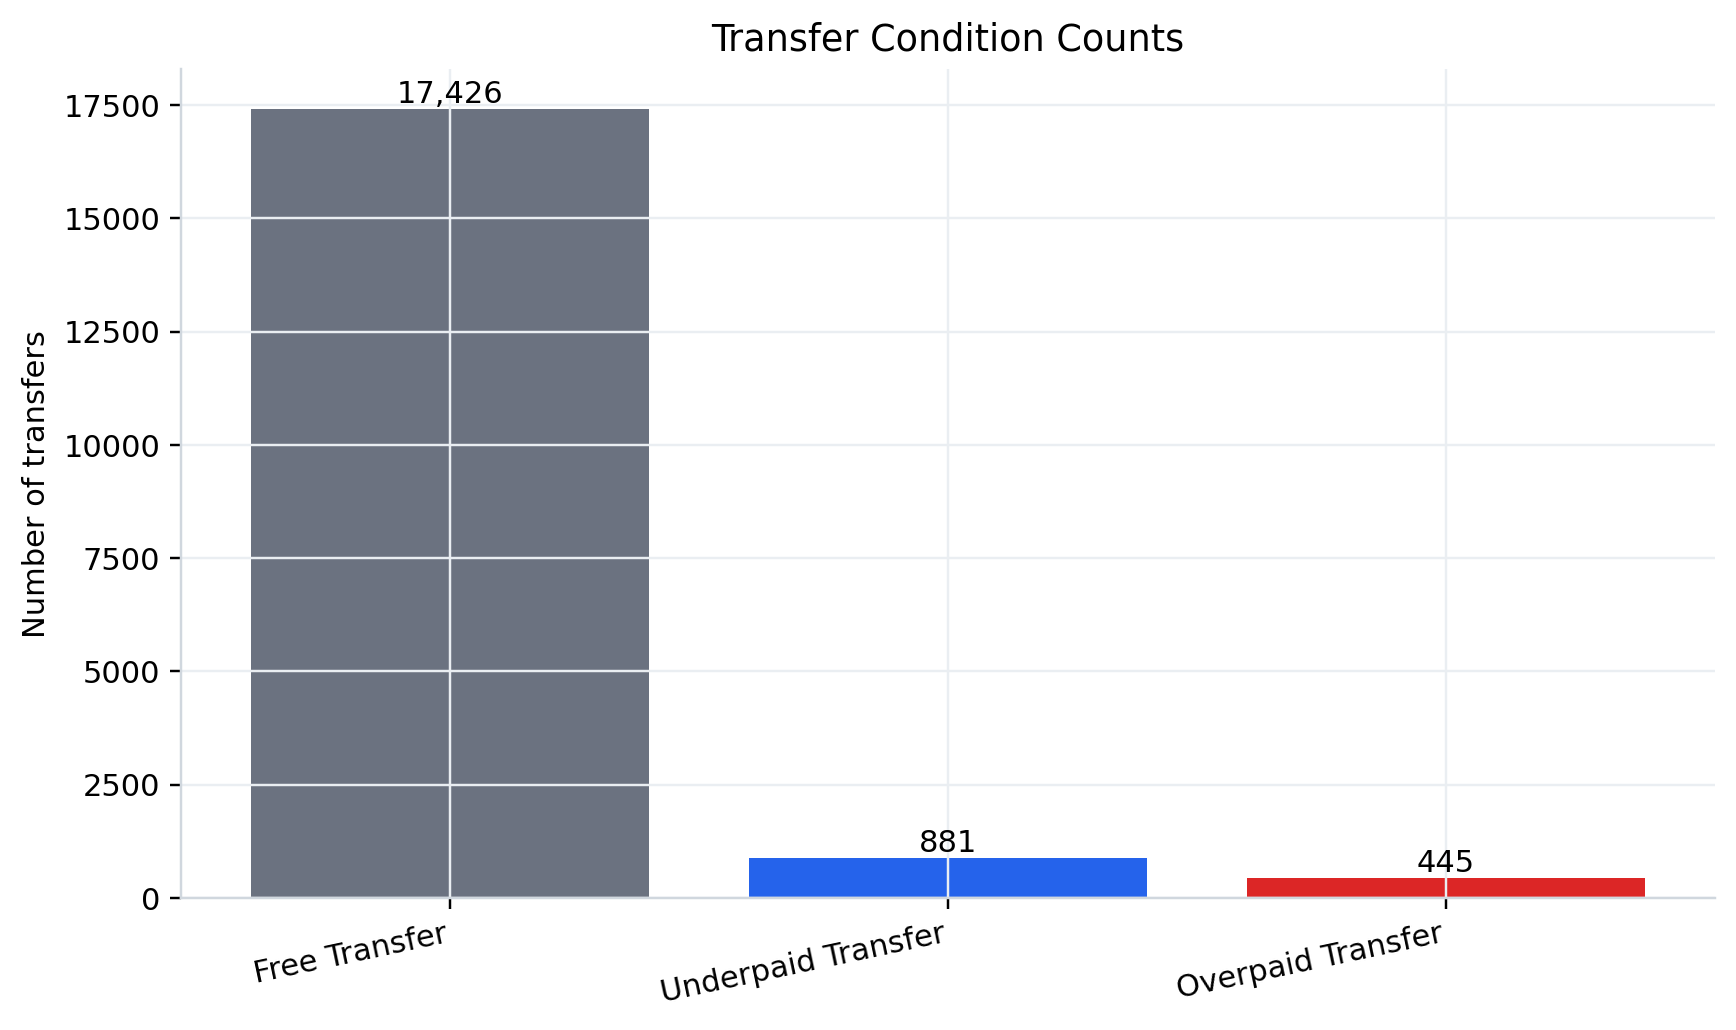
\includegraphics[width=0.82\textwidth]{03_chart_transfer_condition_counts.png}
\caption{Distribution of transfer conditions. Free transfers dominate the dataset, which explains the strong skewness in transfer cost.}
\label{fig:condition_counts}
\end{figure}

\section{Descriptive Patterns by Player Type and Transfer Condition}

The first descriptive pattern is the difference across player types. The dataset contains four main player type groups: defenders, forwards, midfielders, and goalkeepers. Defenders have 5,887 complete records, forwards have 5,610, midfielders have 5,436, and goalkeepers have 1,819. The paid transfer share differs across these groups. Forwards have the highest paid transfer share at 9.1\%, followed by midfielders at 7.0\%, defenders at 6.3\%, and goalkeepers at 3.8\%. Forwards also have the largest mean transfer distance, about 816.6 km.

\begin{figure}[H]
\centering
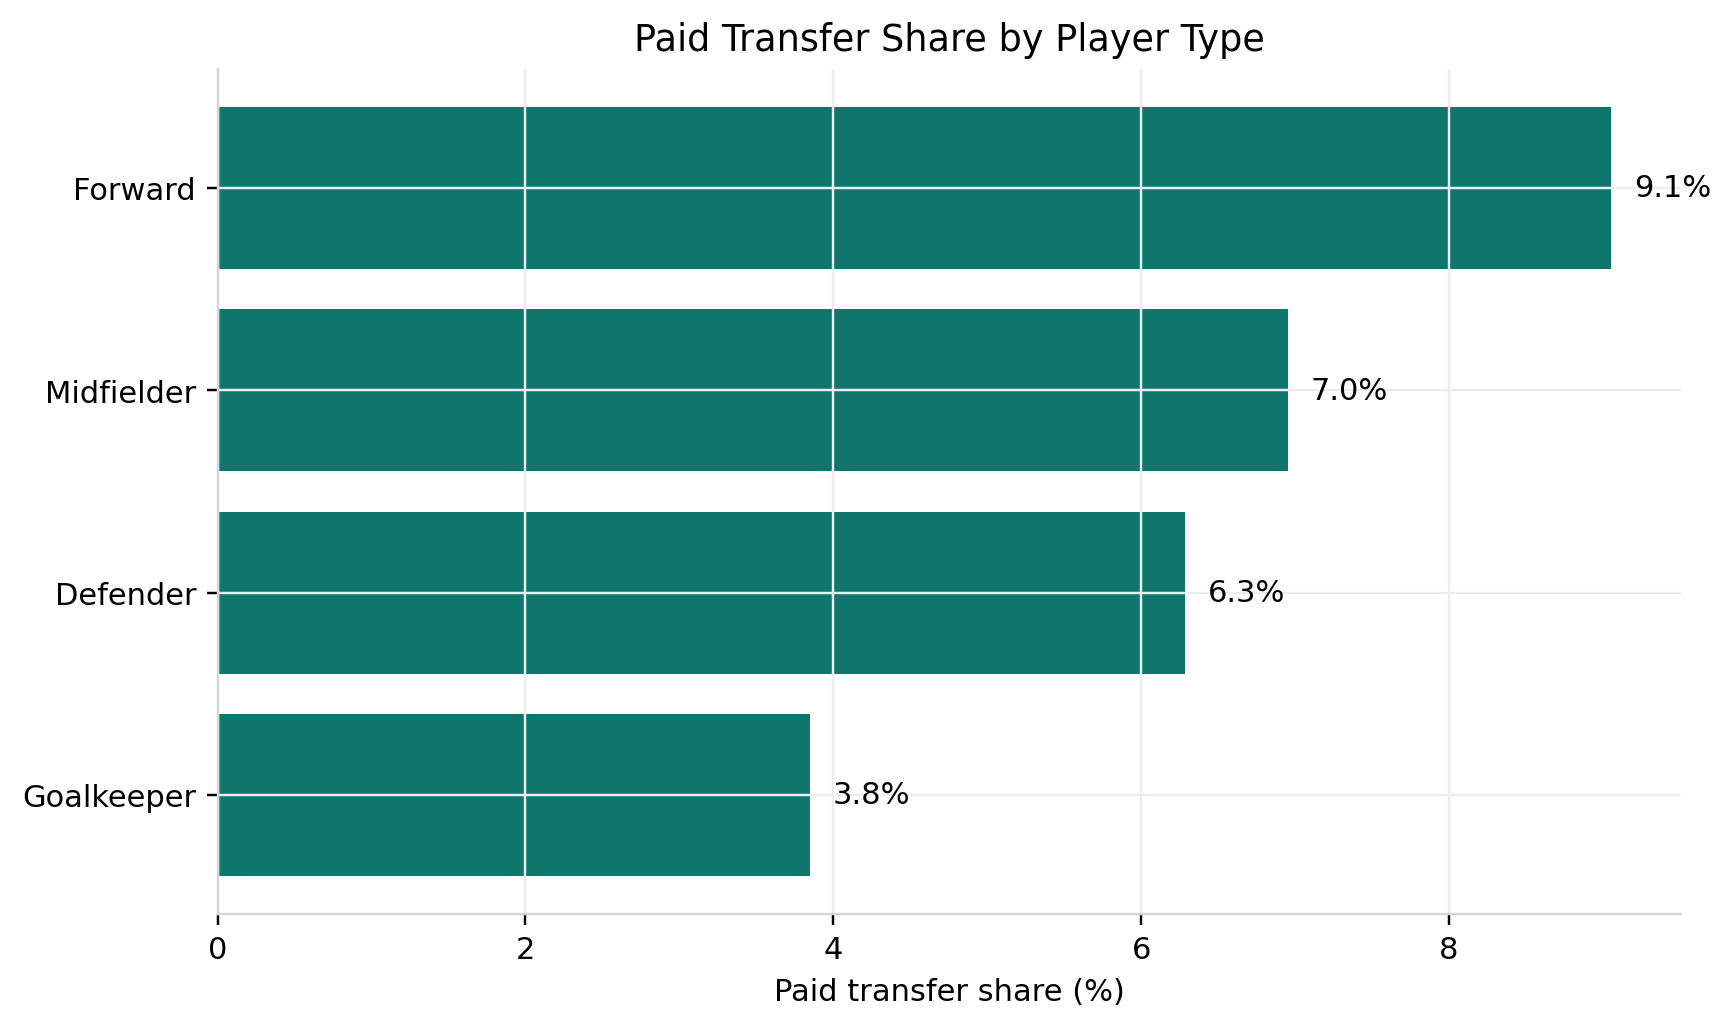
\includegraphics[width=0.82\textwidth]{04_chart_player_type_paid_share.png}
\caption{Paid transfer share by player type. Forwards are more likely to appear in paid transfers than the other player types.}
\label{fig:paid_share}
\end{figure}

This descriptive result is consistent with the economic intuition of football markets. Forwards are directly linked to goals, entertainment value, and media attention. They may therefore attract more active search across countries and more paid transactions. Goalkeepers, in contrast, are more specialized and limited in team demand, which may lead to a lower paid transfer share.

Transfer condition also reveals an important age pattern. Free transfers have an average age of 25.582 years. Underpaid transfers have an average age of 24.658 years. Overpaid transfers have an average age of 22.813 years. Thus, overpaid transfers are on average younger. This suggests that high relative prices are often connected with future potential rather than only current value.

\section{Covariance Structure and the Wishart Framework}

Multivariate analysis begins with covariance. The covariance matrix describes how variables move together. In this paper, the variables are age, log market value, log cost, relative premium intensity, and transfer distance. The most important observed covariance pattern is the strong relationship between log market value and log cost. In the standardized paid-transfer sample, their covariance is approximately 0.858. Log cost also has a positive covariance of about 0.443 with relative premium intensity. Age has a negative covariance of about -0.313 with relative premium intensity.

These values show that transfer cost is not isolated. It moves together with market value and premium intensity, while premium intensity is partly connected with age. Younger players can receive higher relative premiums because clubs are not only buying current ability, but also future development, resale possibility, and scarcity.

The Wishart distribution gives the theoretical background for covariance-based multivariate analysis. If a random sample is drawn from a $p$-dimensional multivariate normal distribution with covariance matrix $\Sigma$, then:

\begin{equation}
(n-1)S \sim W_p(n-1, \Sigma),
\end{equation}

where $S$ is the sample covariance matrix and $W_p$ denotes the $p$-dimensional Wishart distribution. This result is a multivariate extension of the chi-square distribution. In single-variable statistics, sample variance is related to a chi-square distribution. In multivariate statistics, the sample covariance matrix is related to a Wishart distribution.

The Wishart framework matters because PCA, Mahalanobis distance, and Hotelling's $T^2$ all depend on covariance matrices. PCA uses the eigenvalues and eigenvectors of a covariance or correlation matrix. Mahalanobis distance uses the inverse covariance matrix. Hotelling's $T^2$ uses a pooled covariance matrix to compare two mean vectors. Even though these methods answer different questions, they share the same mathematical foundation.

The data in this paper do not perfectly satisfy multivariate normality, so the Wishart distribution should not be interpreted as a strict data-generating truth. Instead, it is used as a theoretical reference point. It explains why the covariance matrix is central and why checking normality is necessary before interpreting classical multivariate procedures.

\section{Principal Component Analysis}

Principal component analysis is used to reduce correlated variables into a smaller number of uncorrelated components. In this paper, PCA answers the question: can age, log market value, log cost, premium intensity, and distance be summarized by a few interpretable transfer-market dimensions?

The PCA results show that the first principal component has an eigenvalue of 1.9658 and explains 39.29\% of the total variance. The second component explains 27.45\%. Together, the first two components explain 66.73\% of the variance. The first three components explain 86.54\%. Thus, most of the multivariate structure can be summarized by three dimensions.

\begin{figure}[H]
\centering
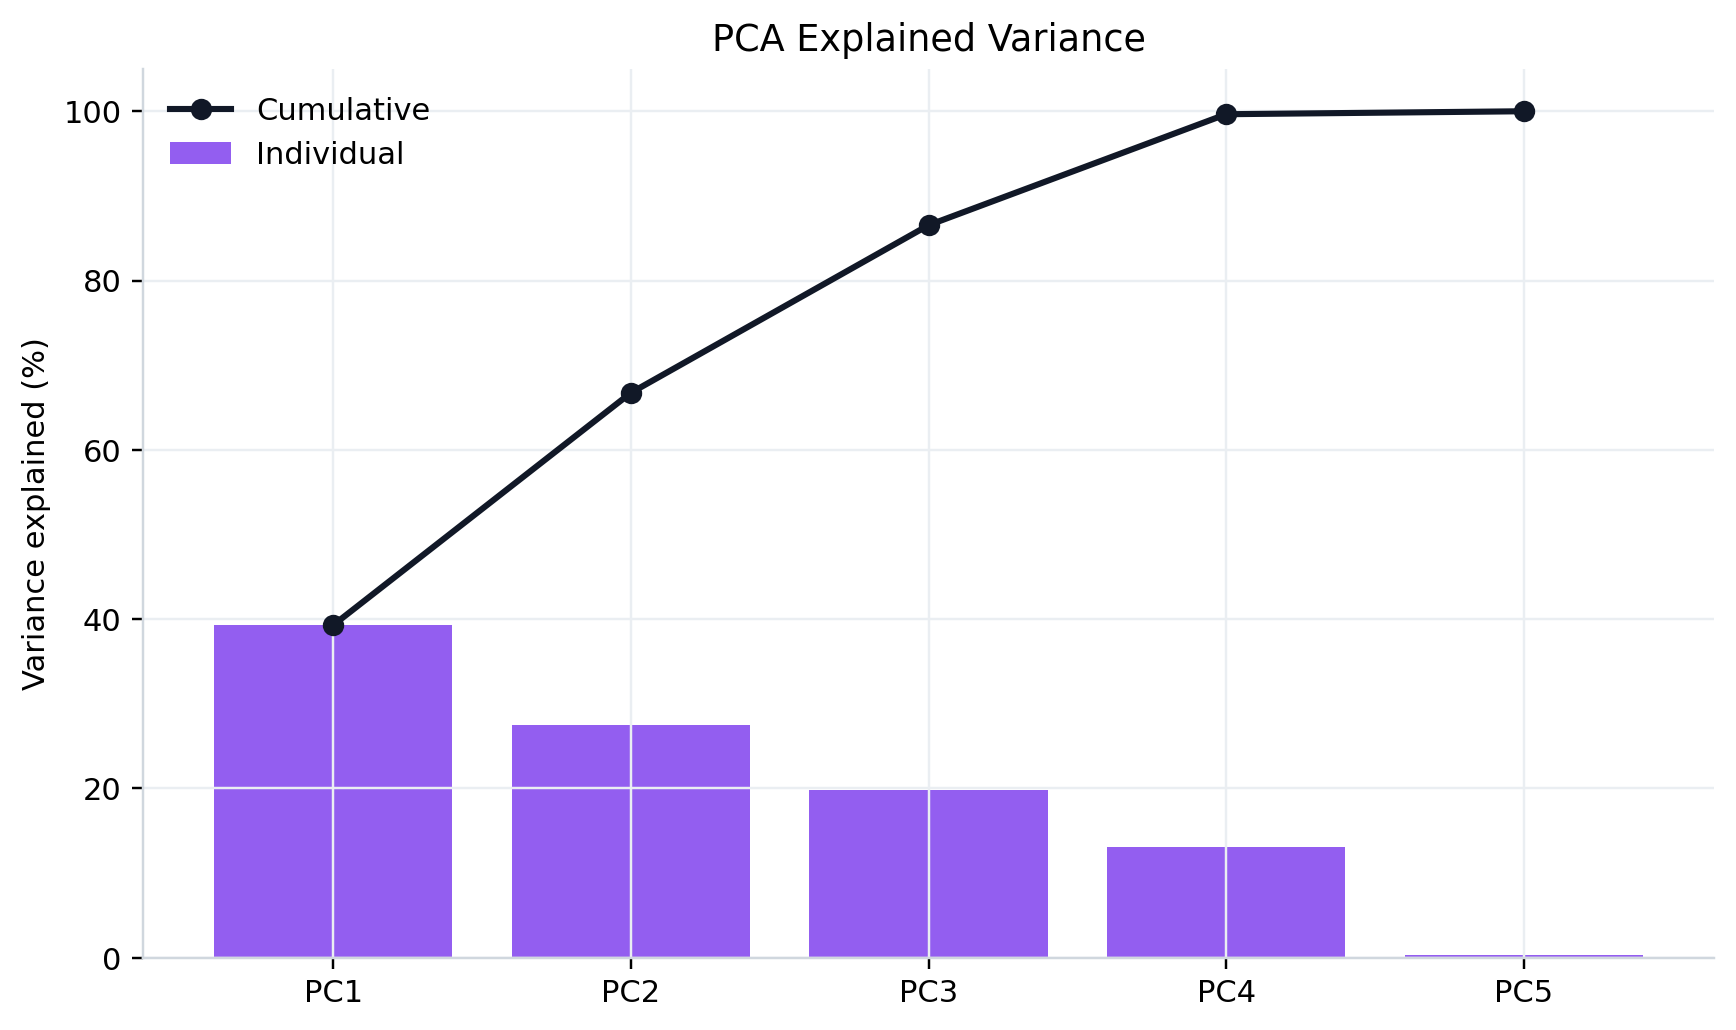
\includegraphics[width=0.82\textwidth]{05_chart_pca_explained_variance.png}
\caption{Explained variance from PCA. The first three principal components capture most of the multivariate variation.}
\label{fig:pca_variance}
\end{figure}

The loadings help interpret the components. The first component is mainly driven by log cost, log market value, and premium intensity. The loading for log cost is 0.7074, and the loading for log market value is 0.6187. Therefore, PC1 can be interpreted as a price and value scale. Transfers with high PC1 scores tend to involve higher market values and higher transfer costs.

The second component contrasts age and premium intensity. Age has a loading of 0.6747, while premium intensity has a loading of -0.6349. This component can be interpreted as an age-versus-premium axis. It separates older, lower-premium transfers from younger, higher-premium transfers. The third component is mainly geographical, with distance having a loading of 0.9640. This component captures transfer mobility.

\begin{figure}[H]
\centering
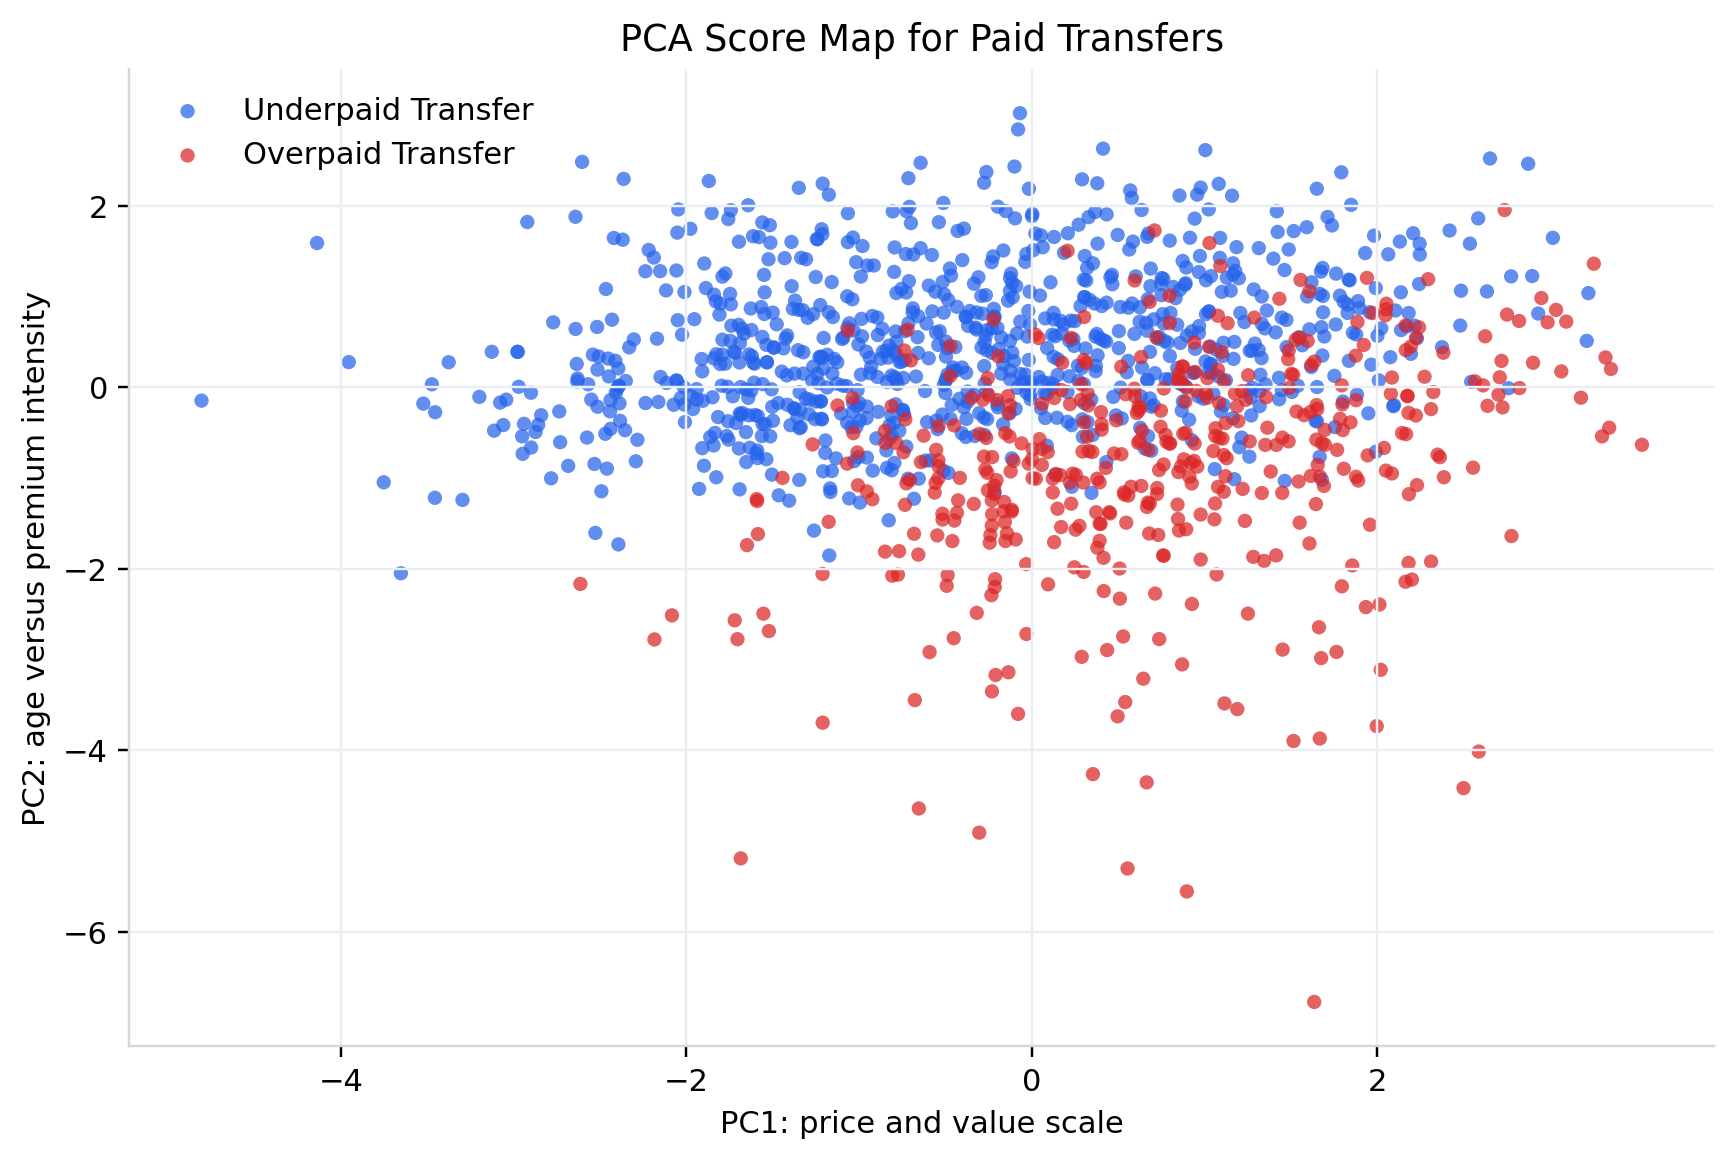
\includegraphics[width=0.82\textwidth]{06_chart_pca_scores_by_condition.png}
\caption{PCA score map for paid transfers. PC1 represents price and value scale, while PC2 represents age versus premium intensity.}
\label{fig:pca_scores}
\end{figure}

The interpretation of PCA is important. PCA does not prove causality. It does not show that age causes premiums or that distance causes high transfer fees. Instead, it reveals the major directions of variation in the data. The football market can be described by at least three dimensions: how expensive the transfer is, whether the transfer is connected to youth and relative premium, and how geographically mobile the player is.

\section{Multivariate Normality Diagnostics}

Many classical multivariate methods are connected to the multivariate normal distribution. Therefore, it is necessary to check whether the data are close to normal. This paper uses Mardia's multivariate skewness and kurtosis tests. The paid-transfer sample produces Mardia skewness of 39.0152, with a p-value close to zero. Mardia kurtosis is 95.6376, also with a p-value close to zero.

These results reject multivariate normality. This is not surprising. Transfer data are highly skewed and heavy-tailed. Most transfers are small or free, but a few transfers are very expensive. Some young players have unusually high fees relative to their market values, while some high-value players move at unusually low costs. International movement also creates unusual distance patterns.

The rejection of multivariate normality is itself an important empirical finding. It means that normal theory should be used carefully. In this paper, multivariate normality is treated as a theoretical benchmark rather than a strict assumption. The methods remain useful as descriptive and diagnostic tools, but p-values and thresholds should be interpreted with caution.

\section{Mahalanobis Distance and Joint Outlier Detection}

Single-variable outlier detection is limited. A player may not have the highest transfer fee, the youngest age, or the longest distance, but the combination of these variables may still be unusual. Mahalanobis distance solves this problem by measuring distance from the multivariate center while accounting for covariance.

For an observation $x$, the squared Mahalanobis distance is:

\begin{equation}
D^2 = (x-\bar{x})'S^{-1}(x-\bar{x}),
\end{equation}

where $\bar{x}$ is the sample mean vector and $S^{-1}$ is the inverse sample covariance matrix. The use of $S^{-1}$ is crucial because it adjusts for correlation among variables. Variables that move together are not counted as independent sources of unusualness.

In the five-dimensional paid-transfer sample, the 97.5\% chi-square threshold is 12.8325, and the 99\% threshold is 15.0863. In the actual data, 5.96\% of records exceed the 97.5\% threshold, and 4.00\% exceed the 99\% threshold. These percentages are higher than expected under ideal multivariate normality, again reflecting heavy tails.

\begin{figure}[H]
\centering
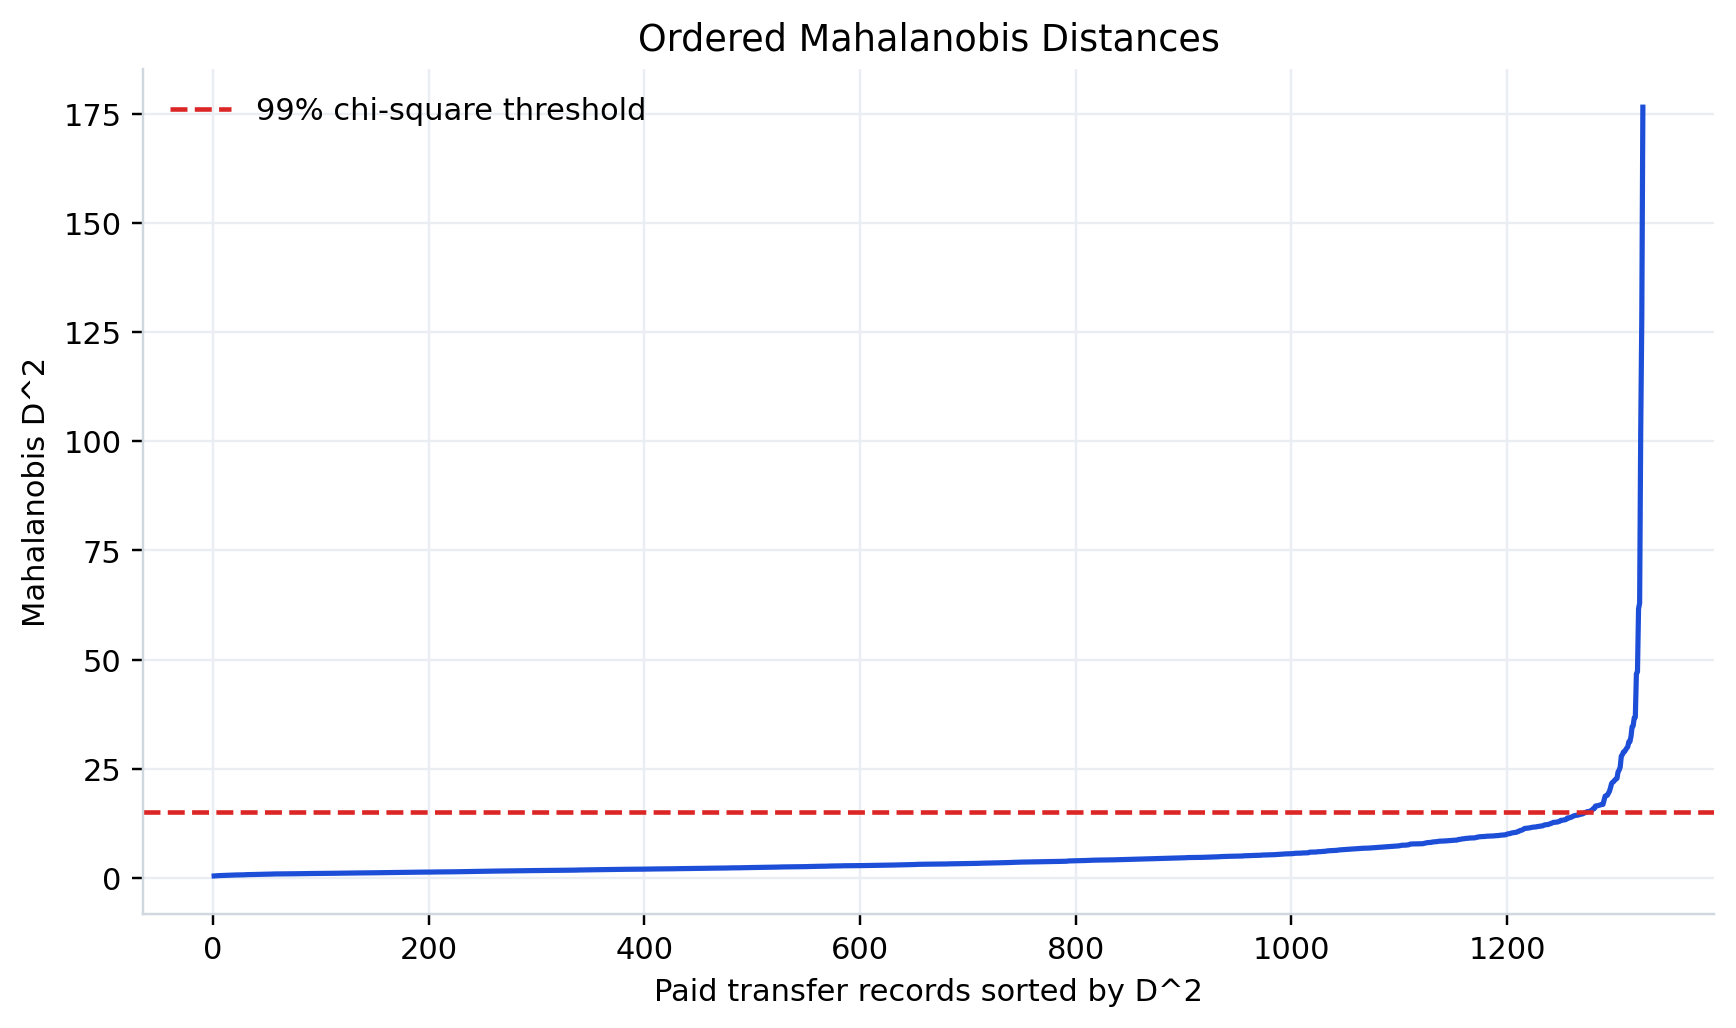
\includegraphics[width=0.82\textwidth]{07_chart_mahalanobis_distance.png}
\caption{Ordered Mahalanobis distances for paid transfers. The high upper tail indicates several transfers with unusual joint profiles.}
\label{fig:mahalanobis}
\end{figure}

The largest Mahalanobis distances include cases such as Kofi Balmer, Arthur Chaves, Roman Evgenjev, Alejandro Pozuelo, and Cesare Casadei. These observations are not necessarily the largest transfers by fee alone. Instead, they are unusual because their age, market value, cost, premium intensity, and transfer distance jointly deviate from the normal market pattern. This is exactly the advantage of Mahalanobis distance: it identifies unusual combinations rather than only extreme single values.

\section{Hotelling's \texorpdfstring{$T^2$}{T2}: Paid and Free Transfers}

Paid and free transfers obviously differ in cost. However, a more meaningful question is whether they differ in their complete multivariate profiles. Hotelling's $T^2$ test is the multivariate extension of the two-sample $t$ test. It tests whether two groups have the same mean vector.

The test uses four standardized variables: age, log market value, log cost, and transfer distance. The null hypothesis is:

\begin{equation}
H_0: \mu_{\text{paid}} = \mu_{\text{free}}.
\end{equation}

The alternative hypothesis is that the two mean vectors are different. The test result is:

\begin{equation}
T^2 = 1{,}113{,}386.6849,\quad
F = 278{,}302.1358,\quad
p \approx 0.
\end{equation}

Therefore, the null hypothesis is rejected. Paid and free transfers have significantly different multivariate mean profiles.

The direction of the difference is also important. The standardized mean age for paid transfers is -0.3133, compared with 0.0238 for free transfers. Thus, paid transfers are younger on average. The standardized mean of log market value is 1.8552 for paid transfers and -0.1412 for free transfers. The standardized mean of log cost is 3.5937 for paid transfers and -0.2735 for free transfers. The standardized mean of distance is 0.5450 for paid transfers and -0.0415 for free transfers.

\begin{figure}[H]
\centering
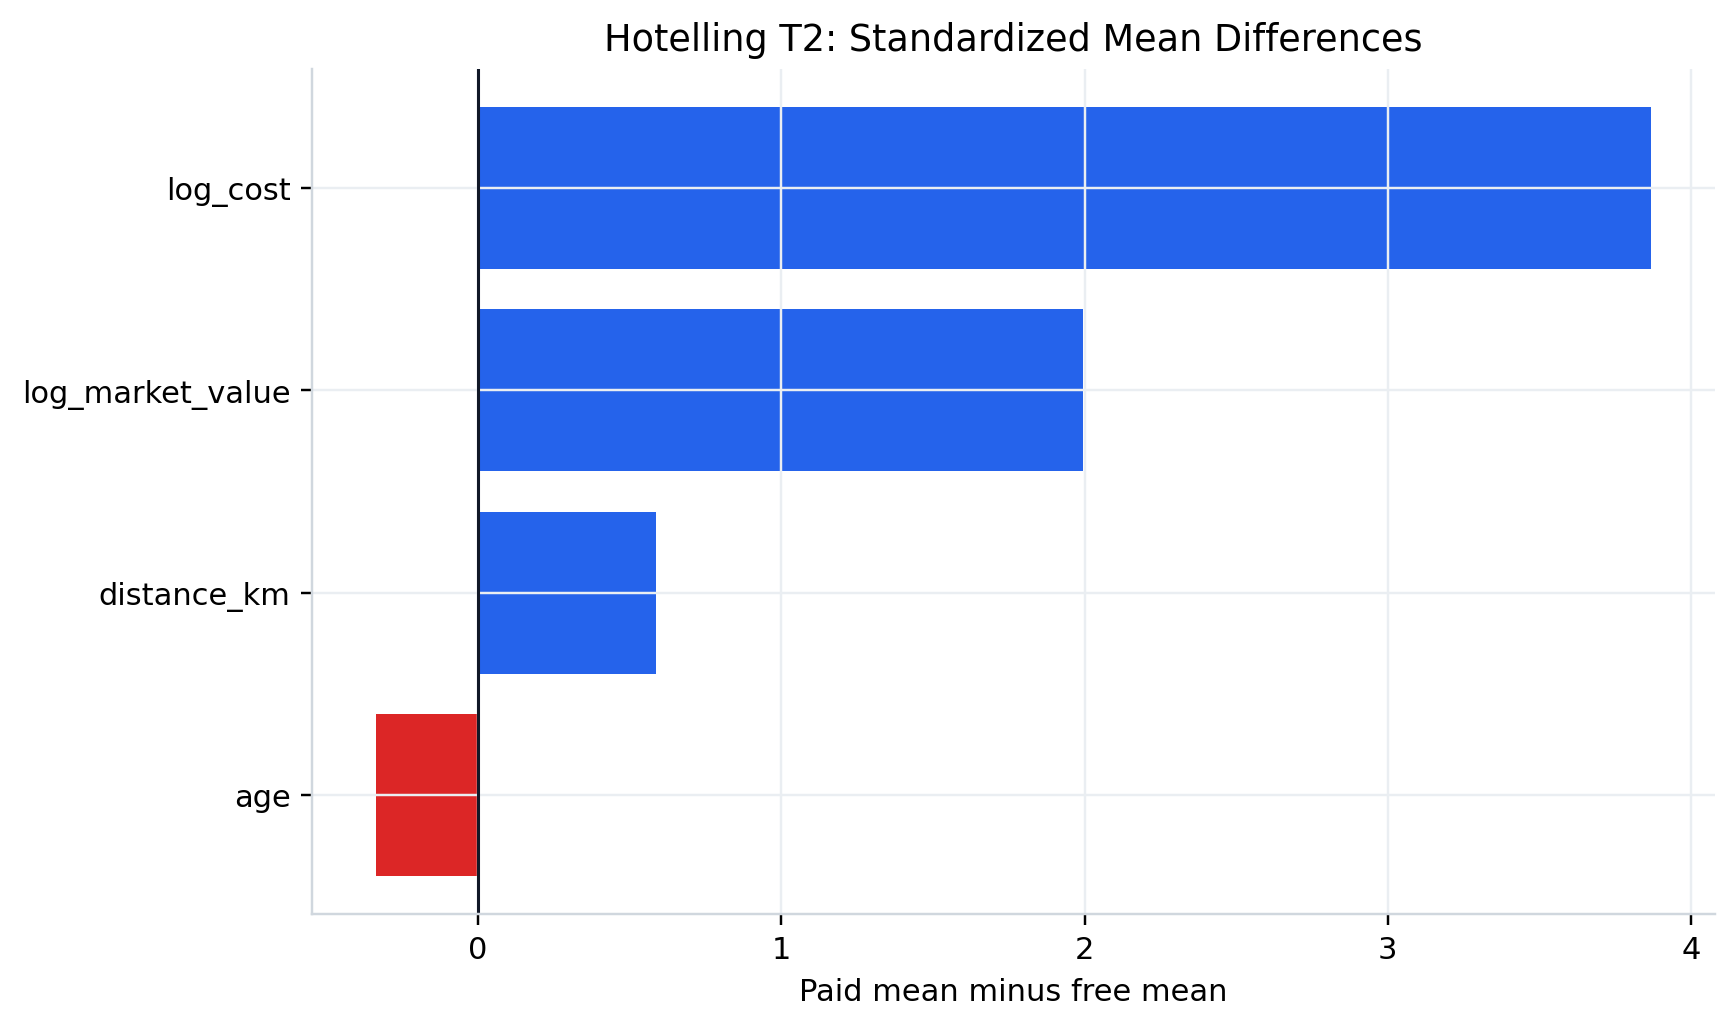
\includegraphics[width=0.82\textwidth]{08_chart_hotelling_mean_differences.png}
\caption{Standardized mean differences used in the Hotelling's $T^2$ comparison. Paid transfers are younger, higher in market value, higher in cost, and more geographically mobile.}
\label{fig:hotelling}
\end{figure}

These results show that paid transfers are not merely free transfers with positive fees. They represent a different market mechanism. Clubs tend to pay fees for younger players, players with higher market value, and players who move across greater distances. Free transfers represent a lower-cost mobility mechanism, while paid transfers represent more active market selection.

\section{MANOVA and Player Type Differences}

The final question is whether different player types have different multivariate transfer profiles. Football positions are not identical market goods. Forwards are often valued for goals, visibility, and entertainment. Midfielders are valued for control and connection. Defenders are valued for stability and defensive structure. Goalkeepers are specialized and have a different demand pattern.

MANOVA tests whether the mean vectors of several groups are equal. In this paper, the dependent variables are age, log market value, log cost, and distance. The grouping variable is player type. The null hypothesis is:

\begin{equation}
H_0: \mu_{\text{Forward}}
= \mu_{\text{Midfielder}}
= \mu_{\text{Defender}}
= \mu_{\text{Goalkeeper}}.
\end{equation}

The result gives Wilks' Lambda of 0.9551, a Bartlett approximate chi-square statistic of 60.7370, 12 degrees of freedom, and a p-value close to zero. The null hypothesis is rejected. Player types have significantly different multivariate transfer profiles.

\begin{figure}[H]
\centering
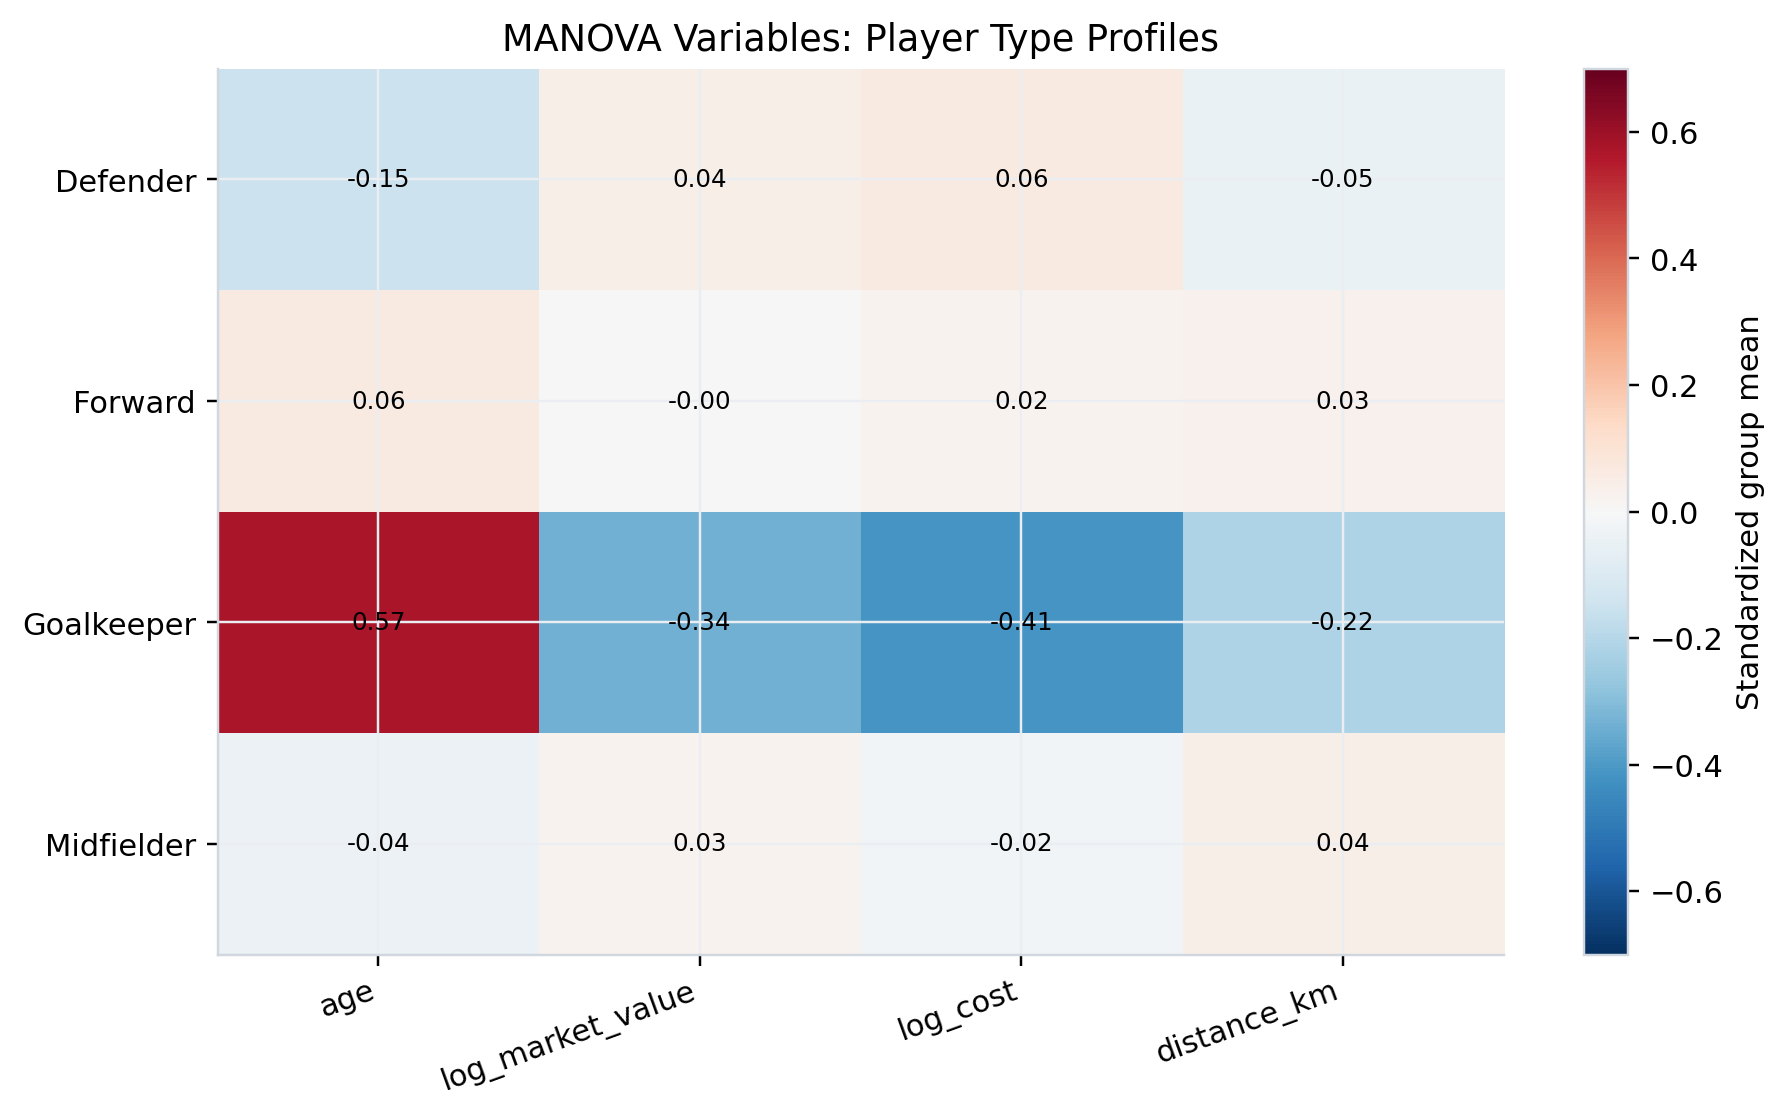
\includegraphics[width=0.82\textwidth]{09_chart_player_type_profiles.png}
\caption{Standardized player type profiles for the MANOVA variables. The player types differ in their joint transfer characteristics.}
\label{fig:manova}
\end{figure}

This result supports the idea that player type is not only a descriptive label. It is connected with the structure of the transfer market. Forwards have the highest paid transfer share and the largest mean distance. Goalkeepers have the lowest paid transfer share and a lower mean distance. Defenders and midfielders are between these two cases. The market appears to treat different functional roles differently.

\section{Discussion}

The methods used in this paper are connected by the covariance structure of the data, but each method solves a different problem. PCA solves the problem of dimensionality. Instead of interpreting five correlated variables separately, PCA identifies broader market dimensions. In this dataset, the main dimensions are price and value scale, age versus premium intensity, and geographical mobility.

The Wishart framework explains why covariance matters. Under multivariate normality, the sample covariance matrix is linked to the Wishart distribution. Even though the data reject strict multivariate normality, the framework still explains why covariance-based methods are mathematically connected.

Mardia's test solves the assumption-checking problem. It shows that football transfer data are not close to multivariate normal. This prevents a careless interpretation of classical methods. The data contain strong skewness and heavy tails because the market includes many free transfers and a small number of extreme paid transfers.

Mahalanobis distance solves the outlier problem. It identifies transfers that are unusual in a joint sense, not only transfers with the highest fees. Hotelling's $T^2$ solves the two-group comparison problem by showing that paid and free transfers differ in their mean vector. MANOVA solves the multi-group comparison problem by showing that different player types have significantly different transfer profiles.

Together, these methods show that football transfer pricing is not one-dimensional. The fee is only one part of a broader multivariate profile. Clubs appear to pay for combinations of youth, value, role, and mobility.

\section{Limitations}

This analysis has several limitations. First, free transfers dominate the dataset. Although logarithmic transformations reduce skewness, they cannot remove the heavy-tailed nature of the market. Second, the dataset contains transfer information but not detailed match performance, injuries, contract length, agent influence, club financial constraints, or tactical fit. Therefore, the analysis should not be interpreted as a full causal model of transfer fees.

Third, the transfer condition variable may partly depend on the relationship between market value and cost. It should therefore be interpreted carefully and not treated as a completely external label. Fourth, geographical distance is calculated from country-level or location-level coordinates. It is a useful proxy for mobility, but it does not fully measure cultural distance, league similarity, scouting cost, or negotiation difficulty.

For these reasons, the goal of the paper is not perfect prediction. The goal is to show how multivariate statistics can organize and explain the structure of football transfer data.

\section{Conclusion}

Football transfer data form a clear multivariate statistical problem. Transfer fees are connected with age, market value, premium intensity, distance, and player type. PCA shows that the main structure can be summarized by price and value scale, age versus premium intensity, and geographical mobility. Mardia's test rejects multivariate normality, showing that the market has strong skewness and heavy tails. Mahalanobis distance identifies unusual transfers based on joint profiles. Hotelling's $T^2$ shows that paid and free transfers differ significantly in their multivariate means. MANOVA shows that forwards, midfielders, defenders, and goalkeepers have significantly different transfer profiles.

The overall conclusion is that football clubs do not buy a single variable. They buy a bundle of market attributes. Younger players, higher-value players, more mobile players, and players in certain functional roles are more likely to enter the paid transfer market. Free transfers represent a different, lower-cost mobility mechanism. Multivariate statistics are useful because they convert a complex transaction table into an interpretable structure of market behavior.

\end{document}
